\section{Affine Indexabbildungen} \label{sec:indextransformationen}

Sei nun $M = \left( x^{ij} \right)_{i,j \in \mathbb{Z}}$ die zu betrachtende unendliche Matrix. Da für die Variable $x$ invertierbare Elemente eines endlichen Körpers $\field{p}[n]$ eingesetzt werden, sind die Minoren von $M$ Polynome aus $\field{p}[n]^\times [X]$. Eine Nullstelle $a \in \field{p}[n]^\times$ eines Minors führt zu einer Submatrix von $M$, die nach Substitution von $a$ nicht invertierbar ist. Die Submatrizen werden mit jeweils zwei endlichen Teilmengen $I,J$ der ganzen Zahlen indiziert. Sei entsprechend $M_{IJ} \coloneqq \left( x^{ij} \right)_{i \in I,j \in J}$.

In diesem Kapitel werden affine Abbildungen $f:\mathbb{Z} \rightarrow \mathbb{Z}, i \mapsto a\cdot i + m$ für $a,m \in \mathbb{Z}$ auf die Indexmengen $I,J \subseteq \mathbb{Z}$ angewendet. Dadurch wird zum Beispiel der Zusammenhang zwischen Minoren zweier zueinander verschobener quadratischer Submatrizen untersucht.

Da bei symmetrischen Matrizen die $i$-te Zeile der $i$-ten Spalte entspricht, gilt $M_{IJ} = M_{JI}^T$ für beliebige Indexmengen $I,J \subseteq \mathbb{Z}$. Für gleich mächtige Indexmengen folgt direkt die erste nützliche Eigenschaft, welche auf die weiteren Sätze in diesem Kapitel angewendet werden kann.

\begin{lemma}
    Sei $M = \left( x^{ij} \right)_{i,j \in \mathbb{Z}}$. Seien weiter $I,J \subseteq \mathbb{Z}$ endliche Teilmengen mit $|I|=|J|$. Dann gilt
    \begin{equation*}
        \det{} M_{IJ} = \det M_{JI}.
    \end{equation*}
\end{lemma}

Beginnend bei den affinen Indexabbildungen wird zuerst das Addieren einer Konstanten auf die Indexmengen untersucht. Für eine Menge $I \subseteq \mathbb{Z}$ und ein $m \in \mathbb{Z}$ sei $I+m \coloneqq \{i+m:i\in I\}$. Dies entspricht dem Verschieben der Submatrizen über die Zeilen und Spalten von $M$. Die Minoren von $M_{IJ}$ und $M_{I+m\,J+n}$ hängen wie folgt zusammen:

\begin{satz} \label{satz:translation}
    \sloppy Sei $M = \left( x^{ij} \right)_{i,j \in \mathbb{Z}}$. Seien weiter $I,J \subseteq \mathbb{Z}$ endliche Teilmengen mit ${|I|=|J|=k}$ und $m,n \in \mathbb{Z}$. Dann gilt
    \begin{equation*}
        \det{} M_{I+m\,J+n} = x^{mnk} x^{n(i_1+\cdots +i_k)} x^{m(j_1 +\cdots + j_k)} \det{} M_{IJ}.
    \end{equation*}
\end{satz}

\begin{proof}
    Die Einträge der Matrix $M_{I+m\,J+n}$ haben die Form 
    \begin{equation*}
        x^{(i+m)(j+n)} = x^{ij} \cdot x^{mj} \cdot x^{ni} \cdot x^{mn} 
    \end{equation*} für $i\in I, j\in J$. Mithilfe der Multilinearität der Determinante können für feste Zeilen- und Spaltenindizes konstante Terme ausgeklammert werden.
    \begin{align*}
        \det M_{I+m\,J+n}    &= \det \left(x^{ij} \cdot x^{mj} \cdot x^{ni} \cdot x^{mn} \right)_{i\in I,j\in J} \\ 
                            &= x^{mnk} \det \left(x^{ij} \cdot x^{mj} \cdot x^{ni} \right)_{i\in I,j\in J} \\ 
                            &= x^{mnk} \left( \prod_{i \in I} x^{ni} \right) \left( \prod_{j \in J} x^{mj}\right)  \det \left(x^{ij}\right)_{i\in I,j\in J} \\
                            &= x^{mnk} x^{n(i_1 +\cdots +i_k)} x^{m(j_1+\cdots +j_k)}\det M_{IJ}.
    \end{align*}
\end{proof}

Da der Vorfaktor $x^{mnk} x^{n(i_1 +\cdots +i_k)} x^{m(j_1+\cdots +j_k)}$ selbst keine Nullstellen in $\field{p}[n]^\times$ besitzt, haben demnach die Minoren zweier zueinander verschobener Submatrizen dieselben Nullstellen. Ist andersherum betrachtet eine Nullstelle $a$ von $\det M_{IJ}$ bekannt, ist $a$ ebenfalls Nullstelle von $\det M_{I+m\,J+n}$ für alle $m,n \in \mathbb{Z}$. Der Satz zeigt zudem, dass die Nullstellen ausschließlich von den Abständen der Indizes in $I$ und $J$ abhängen und nicht von einer Verschiebung innerhalb von $M$. Somit kann es sich anbieten, nur normalisierte Indexmengen zu betrachten, für die $\min(I) = \min(J) = 0$ gilt.

Als Nächstes wird die Multiplikation der Indexmengen mit einer Konstanten untersucht. Für eine Menge $I \subseteq \mathbb{Z}$ und ein $a \in \mathbb{Z}$ sei $aI \coloneqq \{ai:i\in I\}$. Die Minoren von $M_{IJ}$ und $M_{aI\,bJ}$ hängen wie folgt zusammen:

\begin{satz} \label{satz:skalierung}
    \sloppy Sei $M = \left( x^{ij} \right)_{i,j \in \mathbb{Z}}$. Seien weiter $I,J \subseteq \mathbb{Z}$ endliche Teilmengen mit ${|I|=|J|=k}$ und $a,b \in \mathbb{Z}\setminus\{0\}$. Dann gilt
    \begin{equation*}
        \left( \det{} M_{aI\,bJ} \right) (x) = \left( \det{} M_{IJ} \right) (x^{ab}).
    \end{equation*}
\end{satz}

\begin{proof}    
    \begin{align*}
        M_{aI\,bJ}   &= \left(x^{ai\cdot bj}\right)_{i\in I,j\in J} \\
                    &= \left((x^{ab})^{ij}\right)_{i\in I,j\in J}
    \end{align*}

    Die Matrix $M_{aI\,bJ}$ weist somit dieselbe Struktur auf wie $M_{IJ}$. Anstelle von $x$ besitzt $M_{aI\,bJ}$ Variablen der Form $x^{ab}$. Durch Substitution von $x$ durch $x^{ab}$ lässt sich der Minor $\det M_{aI\,bJ}$ aus $\det M_{IJ}$ gewinnen.
\end{proof}

Aus dem gezeigten Satz folgt direkt, dass $\det{} M_{IJ}$ und $\det{} M_{-I\,-J}$ die gleichen Polynome sind und entsprechend die gleichen Nullstellen besitzen. Ist andersherum betrachtet eine Nullstelle $a$ von $\det M_{IJ}$ bekannt, so ist $a^{-1}$ Nullstelle von $\det M_{-I\,J}$ und $\det M_{I\,-J}$.

Die \Cref{satz:translation,satz:skalierung} lassen sich im folgenden Korollar zusammenführen.

\begin{korollar}
    \sloppy Seien $M = \left( x^{ij} \right)_{i,j \in \mathbb{Z}}$ und $I,J \subseteq \mathbb{Z}$ endliche Teilmengen mit ${|I|=|J|=k}$. Seien weiter $m,n \in \mathbb{Z}$ und $a,b \in \mathbb{Z}\setminus\{0\}$. Dann gilt
    \begin{equation*}
        \left( \det{} M_{aI+m\,bJ+n} \right) (x) = x^{mnk} x^{an(i_1+\cdots +i_k)} x^{bm(j_1 +\cdots + j_k)} \left( \det{} M_{IJ} \right) (x^{ab}).
    \end{equation*}
\end{korollar}

\begin{proof}
    \begin{align*}
        \left( \det{} M_{aI+m\,bJ+n} \right) (x)    &= x^{mnk} x^{n(ai_1+\cdots +ai_k)} x^{m(bj_1 +\cdots + bj_k)} \left( \det{} M_{aI\,bJ} \right) (x) \\
                                                    &= x^{mnk} x^{an(i_1+\cdots +i_k)} x^{bm(j_1 +\cdots + j_k)} \left( \det{} M_{aI\,bJ} \right) (x) \\
                                                    &= x^{mnk} x^{an(i_1+\cdots +i_k)} x^{bm(j_1 +\cdots + j_k)} \left( \det{} M_{IJ} \right) (x^{ab}) \\
    \end{align*}
\end{proof}


\sloppy Die Zusammenhänge zwischen transformierten Indexmengen können über Graphen dargestellt werden. Für festes ${a \in \field{p}[n]^\times}$ sei $G_a$ der Graph mit Knotenmenge ${V=\{I \in\mathcal{P}(\mathbb{Z}) : |I| \in \mathbb{N}_+\}}$ und Kantenmenge $E = \{(I,J) : (\det M_{IJ})(a) = 0\}$. Der Graph $G_a$ enthält somit genau dann die Kante $(I,J)$, falls die Submatrix $M_{IJ}(a)$ nicht invertierbar ist.

Aus \Cref{satz:translation} folgt, dass eine Kante $(I,J)$ alle weiteren Kanten $(I+m,J+n)$ für ${m,n\in \mathbb{Z}}$ induziert. Alle Knoten der Form $I+m$ besitzen somit in $G_a$ dieselben adjazenten Knoten. Sei $G[V]$ der durch die Knotenmenge $V$ induzierte Teilgraph von $G$. Das beschriebene Verhalten ist in \Cref{fig:subgraphs} dargestellt. Falls die Indexmengen $I$ und $J$ unterschiedlich sind, ergibt sich der vollständig bipartite Teilgraph aus \Cref{fig:biclique-graph}. Falls jedoch $I$ und $J$ gleich sind, entsteht der in \Cref{fig:complete-graph} dargestellte vollständige Teilgraph, in dem alle Knoten der Form $I+m$ miteinander verbunden sind. 

\begin{figure}[]
    \centering
    \begin{subfigure}[b]{0.47\textwidth}
        \centering
        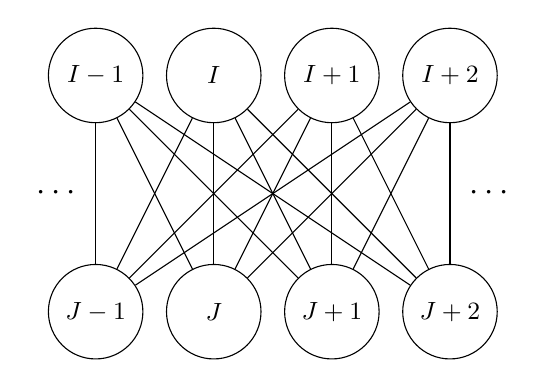
\begin{tikzpicture}[node distance={5mm}, main/.style = {draw, circle, minimum size=1.2cm}]

            \node (D0) at (-0.5,-1.5) {\large $\cdots$};
            \node (D1) at (5,-1.5) {\large $\cdots$};

            % Nodes
            \node[main] (I0) at (0,0) {\small $I-1$};
            \node[main] (I1) at (1.5,0) {\small $I$};
            \node[main] (I2) at (3,0) {\small $I+1$};
            \node[main] (I3) at (4.5,0) {\small $I+2$};
            \node[main] (J0) at (0,-3) {\small $J-1$};
            \node[main] (J1) at (1.5,-3) {\small $J$};
            \node[main] (J2) at (3,-3) {\small $J+1$};
            \node[main] (J3) at (4.5,-3) {\small $J+2$};
    
            % Edges
            \draw (I0) to (J0);
            \draw (I0) to (J1);
            \draw (I0) to (J2);
            \draw (I0) to (J3);
            \draw (I1) to (J0);
            \draw (I1) to (J1);
            \draw (I1) to (J2);
            \draw (I1) to (J3);
            \draw (I2) to (J0);
            \draw (I2) to (J1);
            \draw (I2) to (J2);
            \draw (I2) to (J3);
            \draw (I3) to (J0);
            \draw (I3) to (J1);
            \draw (I3) to (J2);
            \draw (I3) to (J3);
        \end{tikzpicture}
        \caption{${G_a[\{I+m:m\in \mathbb{Z}\} \cup \{J+m:m\in \mathbb{Z}\}]}$ zu Knoten $I \neq J$ mit $(\det M_{IJ})(a) = 0$}
        \label{fig:biclique-graph}
    \end{subfigure}
    \hfill
    \begin{subfigure}[b]{0.47\textwidth}
        \centering
        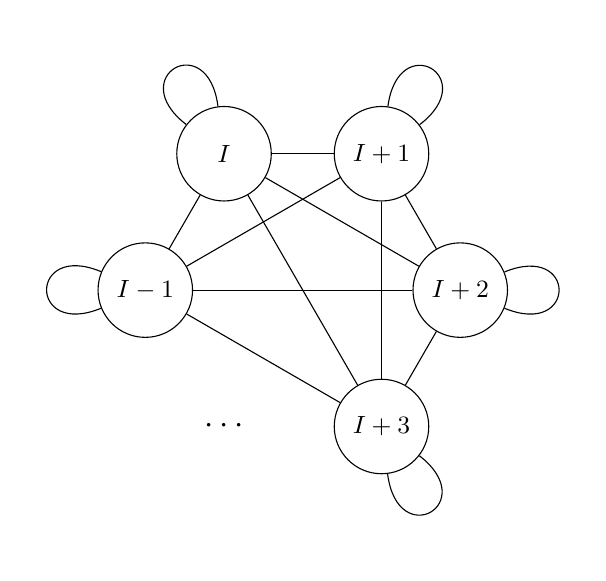
\begin{tikzpicture}[node distance={5mm}, main/.style = {draw, circle, minimum size=1.2cm}]
            % Nodes
            \node[main] (I0) at ({360/6 * 0}: 2cm) {\small $I+2$};
            \node[main] (I1) at ({360/6 * 1}: 2cm) {\small $I+1$};
            \node[main] (I2) at ({360/6 * 2}: 2cm) {\small $I$};
            \node[main] (I3) at ({360/6 * 3}: 2cm) {\small $I-1$};
            \node (D1) at ({360/6 * 4}: 2cm) {\large $\cdots$};
            \node[main] (I4) at ({360/6 * 5}: 2cm) {\small $I+3$};

            \draw (I0) to[loop, out=22.5, in=-22.5, distance=1cm] (I0);         
            \draw (I0) to (I1);
            \draw (I0) to (I2);
            \draw (I0) to (I3);
            \draw (I0) to (I4);            
            \draw (I1) to[loop, out=82.5, in=37.5, distance=1cm] (I1);            
            \draw (I1) to (I2);
            \draw (I1) to (I3);
            \draw (I1) to (I4);
            \draw (I2) to[loop, out=142.5, in=97.5, distance=1cm] (I2);    
            \draw (I2) to (I3);
            \draw (I2) to (I4);
            \draw (I3) to[loop, out=202.5, in=157.5, distance=1cm] (I3);    
            \draw (I3) to (I4);
            \draw (I4) to[loop, out=322.5, in=277.5, distance=1cm] (I4);    
        \end{tikzpicture}
        \caption{${G_a[\{I+m:m\in \mathbb{Z}\}]}$ zum Knoten $I$ mit $(\det M_{II})(a) = 0$}
        \label{fig:complete-graph}
    \end{subfigure}
    \caption{Induzierte unendliche Teilgraphen in $G_a$}
    \label{fig:subgraphs}
\end{figure}

Aus \Cref{satz:skalierung} ergeben sich weitere Symmetrien in $G_a$. Demnach sind die folgenden Aussagen äquivalent

\begin{align*}
    &(\det{} M_{IJ})(a) = 0 \\
    \iff &(\det{} M_{-I\,-J})(a) = 0 \\
    \iff &(\det{} M_{-I\,J})(a^{-1}) = 0 \\
    \iff &(\det{} M_{I\,-J})(a^{-1}) = 0,
\end{align*}
und die induzierten Teilgraphen
\begin{align*}
    &G_a[\{I+m:m\in \mathbb{Z}\} \cup \{J+m:m\in \mathbb{Z}\}], \\
    &G_a[\{-I+m:m\in \mathbb{Z}\} \cup \{-J+m:m\in \mathbb{Z}\}], \\
    &G_{a^{-1}}[\{-I+m:m\in \mathbb{Z}\} \cup \{J+m:m\in \mathbb{Z}\}] \text{ und} \\
    &G_{a^{-1}}[\{I+m:m\in \mathbb{Z}\} \cup \{-J+m:m\in \mathbb{Z}\}]
\end{align*}
isomorph.

Somit induziert die bijektive Abbildung $f:V \to V, I \mapsto -I$ einen nicht trivialen Graphautomorphismus und einen Graphisomorphismus zwischen $G_a$ und $G_{a^{-1}}$.